\section{User Study: Designing \papertitle}
We have used several tools to accomplish the research. On the software side, we have utilized Unity, a game engine software, and the C\# programming language to create prototypes for our \papertitle\ keyboard. On the hardware side, we have used Asus Padfone Infinity mobile phone running Android 4.4. This phone has a 5 inch display. We have decided to use a smartphone first instead of an actual smartwatch because prototyping on a smartphone is faster and more convenient. This is especially true because Unity allows us to make quick designs and upload them into the smartphone. Even though it does not support smartwatches, we can still design a smartwatch screen on Unity and let it mimic the actual size and features on the smartphone.

We have attached this phone to the user’s non-dominant arm where the screen is positioned in landscape orientation, a setup that was also used in Luis et al.’s study \cite{text-entry-on-small-qwerty}. We have rendered a smartwatch screen with a dimension of 29mm x 29mm on the smartphone. Within this 29mm x 29mm smartwatch screen we have positioned the keyboard with a dimension of 25mm x 15mm. This keyboard can fit on most commercially available smartwatches.

\begin{figure*}
\begin{subfigure}{.24\textwidth}
  \centering
  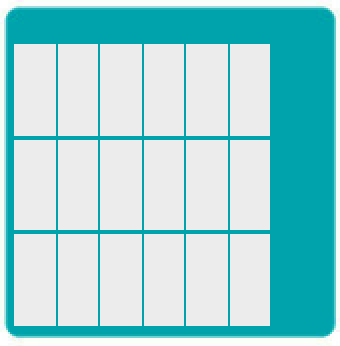
\includegraphics[width=.7\linewidth]{figures/F3-1.png}
  \caption{button shape: 3.9 x 7.8 mm}
  \label{fig:f3a}
  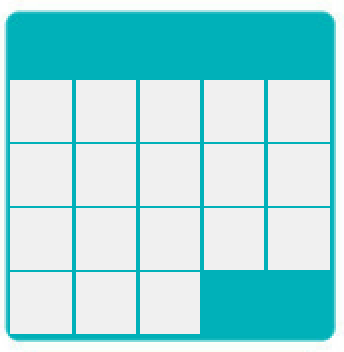
\includegraphics[width=.7\linewidth]{figures/F3-2.png}
  \caption{button shape: 5.5 x 5.5 mm}
  \label{fig:f3b}
\end{subfigure}%
\begin{subfigure}{.24\textwidth}
  \centering
  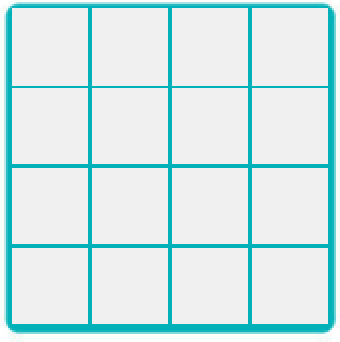
\includegraphics[width=.7\linewidth]{figures/F3-3.png}
  \caption{button size: 7.1 mm}
  \label{fig:f3c}
  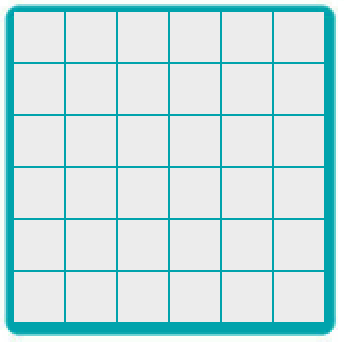
\includegraphics[width=.7\linewidth]{figures/F3-4.png}
  \caption{button size: 4.8 mm}
  \label{fig:f3d}
\end{subfigure}
\begin{subfigure}{.24\textwidth}
  \centering
  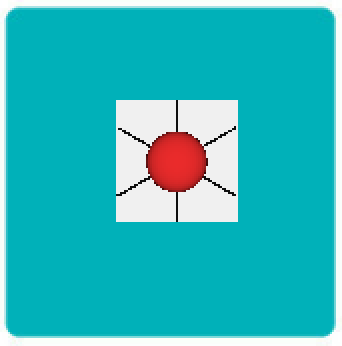
\includegraphics[width=.7\linewidth]{figures/F3-5.png}
  \caption{swipe per button: 7}
  \label{fig:f3e}
  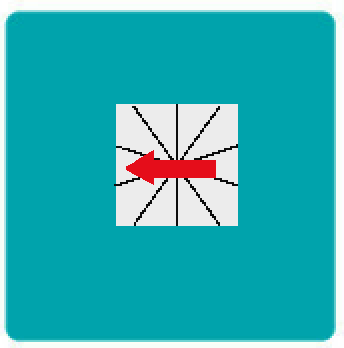
\includegraphics[width=.7\linewidth]{figures/F3-6.png}
  \caption{swipe per button: 10}
  \label{fig:f3f}
\end{subfigure}
\begin{subfigure}{.24\textwidth}
  \centering
  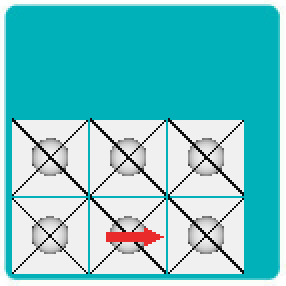
\includegraphics[width=.7\linewidth]{figures/F3-7.png}
  \caption{button layout: \papertitle 5}
  \label{fig:f3g}
  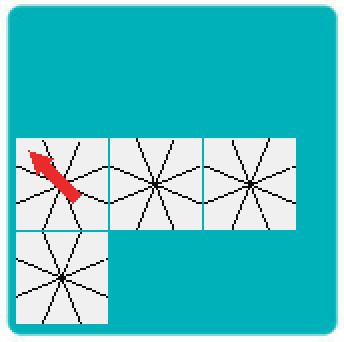
\includegraphics[width=.7\linewidth]{figures/F3-8.png}
  \caption{button layout: \papertitle 8}
  \label{fig:f3h}
\end{subfigure}
\caption{Sample layout of User Study for designing \papertitle (a),(b) button shape test layout. Each layout contains 18 buttons. (c), (d) button size test layout. (e), (f) swipe per button test layout. Each button is 10 mm per side. (e) is 7 swipe button with a highlight circle to instruct user to tap on that button (f) is 10 swipe button with an arrow instruct user to perform left swipe.  (g), (h) button layout test layout. Each layout is confined in a 15 x 25 mm space}
\label{fig:f3}
\end{figure*}

Figure 2 shows some examples of different keyboard layouts that we have tested during our user study. In this test, a single random button will light up in red. A circle in a button can either be lit up red or an arrow will light up. If a circle in the button is highlighted, the user simply needs to tap on the corresponding button. On the other hand, if a highlighted arrow appears, then the user needs to swipe on that button toward the direction indicted by the arrow. For this swipe motion, the finger must press and start from the button with the highlighted arrow. After initiating the swipe the user can let go of the screen anywhere as long as the finger motion follows the direction the highlighted arrow pointing towards.

After the user finished tapping or swiping on a button, a new random button will light up. The user gains a point every time the user taps or swipes on the correct button and towards the correct direction. In case of mistakes, such as missing the highlighted button or not swiping towards the correct direction, would produce a red flash on the screen. The user will not gain any point for any misses. The user must get as many points as possible within a 60 second time frame. After the timer is up, the screen will display the number of hits, the number of total taps and swipes, and the percentage of hits over the total number of taps and swipes.

In this user study for designing \papertitle, we have conducted this test with 12 users with ages ranging from 19 to 35 (7 male and 5 female).

\subsection{Button Shape}
We have decided to make the keyboard buttons square shaped for 3 reasons, inspired by the consideration of I Scott MacKenzie \cite{opti}:
\begin{itemize}
\item[1.]Square or rectangular shaped buttons can be tightly packed together in a grid formation without leaving empty gaps between each button (dead space)
\item[2.]Square shaped buttons are better for touch accuracy compared to rectangular shaped buttons
\item[3.]Square shaped buttons make every swipe direction angles equal. For example, if the aspect ratio for horizontal/vertical were 2, then it would be easier to swipe horizontally than vertically. If, on the other hand, the buttons are square, then swiping horizontally or vertically will have equal accuracy.
\end{itemize}

The second statement above is demonstrated in Lee’s work \cite{performance-of-soft-button}. He showed that square-like buttons (wider button) are more preferable than rectangle-like buttons (narrow buttons). To further study the effect of the role of aspect ratio, we have conducted a user study of button shape on buttons with different aspect ratio but with the same size. Users were asked to tap on a random highlighted button continuously. Figure 2(a) and (b) show the sample test layout.

The result in Figure 3 shows that both error rate and tapping speed will worsen for an aspect ratio different from 1. This suggests that a keyboard design with buttons close to being square shaped is preferred for high speed and low error text entry.

\begin{figure}
  \begin{subfigure}{1\columnwidth}
  \centering
  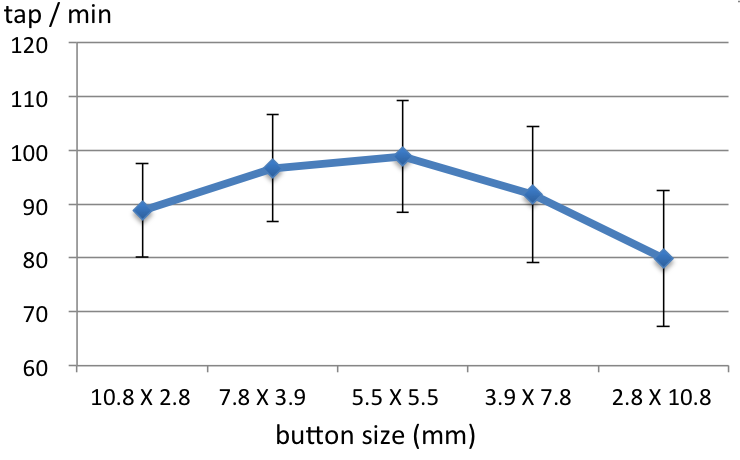
\includegraphics[width=.8\columnwidth]{figures/F4-1.png}
  \caption{}
  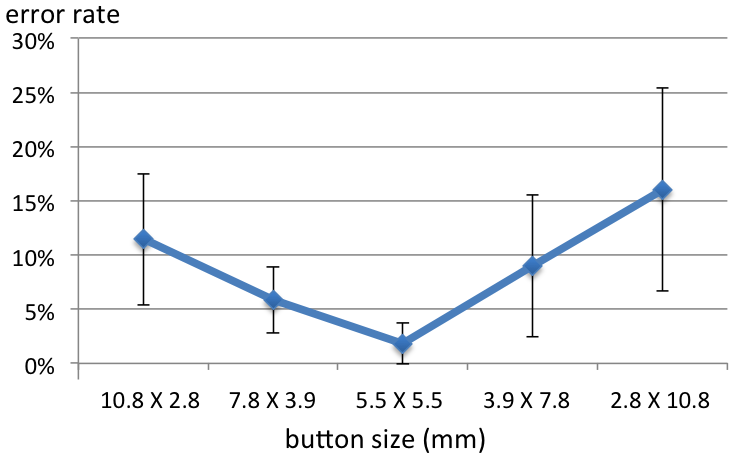
\includegraphics[width=.8\columnwidth]{figures/F4-2.png}
  \caption{}
  \label{fig:f4}
  \end{subfigure}
  \caption{Button shape test result. (a) Tap speed of 12 users (c) Error rate}
\end{figure}

\subsection{Button Size and Swipe per Button}
The size of the keyboard and the number of characters are two constrains that connect the button size and swipes per button. Our final goal was to put 26 possible entries (characters in the alphabet) onto the smartwatch keyboard. That means that if we had a keyboard that heavily relied on using swipe motions instead of using tap motions to select entries on a button, we could have made each button bigger. Therefore, we needed to consider at the same time these two correlated parameters: the number of possible swipe directions per button and the button size. Even if they are dependent on each other, we still had to test them individually in separate experiments to further understand the importance of both parameters.

For the experiment involving button sizes, we created different keyboard designs, each with differently sized buttons. On one hand, having bigger buttons meant that the users had an easier time pressing each of them accurately, but it also meant that we would not be able to fit many buttons on the smartwatch screen. On the other hand, we would be able to place more buttons on the screen if the buttons are small, but it would have meant that the users would have difficulty pressing each button accurately. During the experiment, users were asked to tap on differently sized square buttons similar to the previous tests. We evaluated them on how many correct button presses they made for each of the button sizes. After testing, we asked the user which button size they had trouble tapping on correctly. The results are shown in Figure 4.

\begin{figure}
  \begin{subfigure}{1\columnwidth}
  \centering
  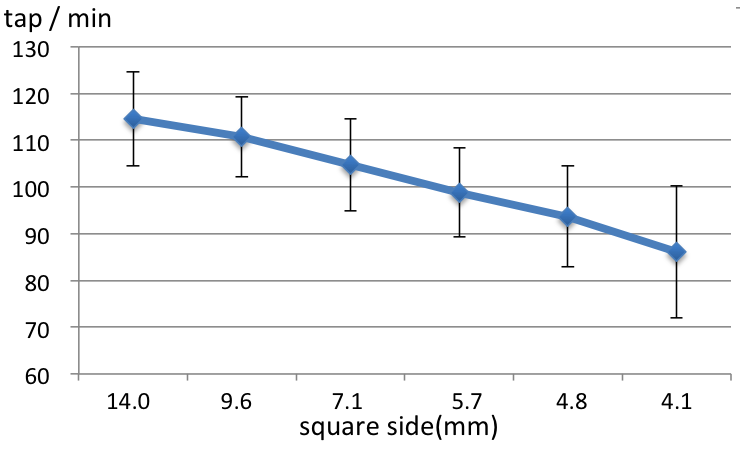
\includegraphics[width=.8\columnwidth]{figures/F5-1.png}
  \caption{}
  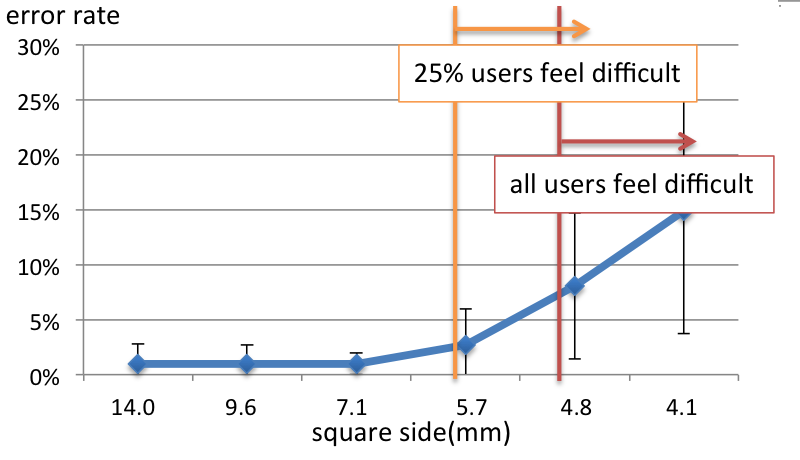
\includegraphics[width=.8\columnwidth]{figures/F5-2.png}
  \caption{}
  \label{fig:f5}
  \end{subfigure}
  \caption{Result of button size test. (a) Tap speed (b) Error rate}
\end{figure}

The results show that the speed decreases steadily as we make the button size smaller. The error rate rises dramatically for button size smaller than 5.7mm x 5.7mm. All the users felt that it was difficult to tap on the correct button with button size smaller than 4.8mm x 4.8mm. About 25\% of the users felt that tapping on 5.7mm x 5.7mm buttons was difficult. It suggests making keyboard buttons at least 5.7mm x 5.7mm large.

Then we designed a test to investigate the accuracy of swipe motions. In this test, a large button is divided into different angle sections. An arrow will randomly light up red and the user is asked to swipe towards the direction the arrow is pointing towards from the center of the button. Different button designs may allow different amounts of swipe directions. The number of swipe directions determines the number of directions the arrow can point. For example, if a button design has 4 swipe directions, it means that the arrow can end up pointing at 4 possible directions: up, down, left, and right. Figure 2 (f) shows a button with 10 swipe directions, meaning the arrow can point towards any of the 10 directions (mixture of left, right, and diagonal swipes). A button with small number of swipe directions would be easier to swipe in the correct direction than ones with a large number. This is because users need to be more precise with the angle of the swipe he or she makes with buttons with more swipe directions. In other words, a button 4 swipe direction has more tolerance in swipe angle than ones with 10 swipe directions. Clearly, we do not want to have too many swipe directions per button, or else the keyboard will be difficult to use.

Users were asked to swipe to towards a random chosen direction on a 10 x 10 mm button. Since we consider both vertical and horizontal symmetry, only even swipe numbers are taken into account. In addition, there are many works that combine tap with swipe for text entry buttons. Therefore, we also consider every even swipe with an additional tap as a candidate \papertitle\ button. After this test, we also asked the user to choose buttons that are hard to follow correctly. Note that the odd number swipe represents its lower even number swipe plus one tap. The sample layout is in Figure 2(e), (f). The results of the experiment are shown in Figure 5.

Figure 5(a) shows that the swipe speed is about 90 swipes per minute on average, and the swipe speed is almost independent to swipes per button. But the error rate and user experience is highly correlated with the number of swipes per button. The error rate rises when the number of swipes per button is larger than 8 swipes. Notice that even though the error rate is low for 6 swipes, 17\% of the users felt that it was difficult to swipe correctly with this number of swipe directions. Moreover, the layout with tap and swipe has higher accuracy (???) than the group with swipe only. It suggests that the combination of 2 different types of movements (tap and swipe) might increase the possibility of making errors. This inconsistency between tap and swipe is also reported by 25\% of users. 

\begin{figure}
  \begin{subfigure}{1\columnwidth}
  \centering
  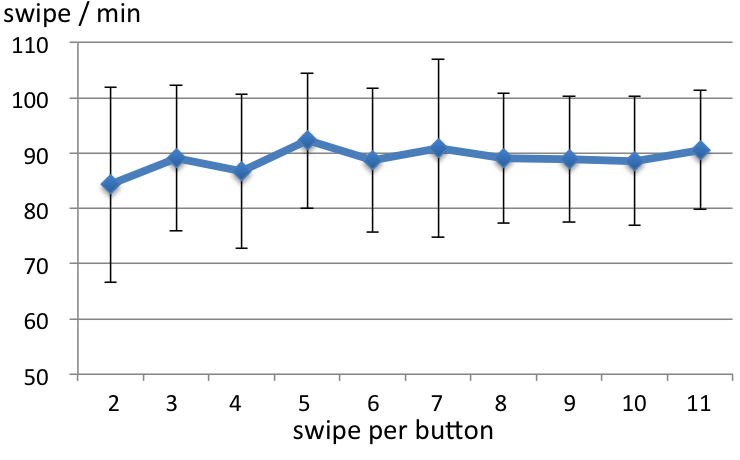
\includegraphics[width=.8\columnwidth]{figures/F6-1.png}
  \caption{}
  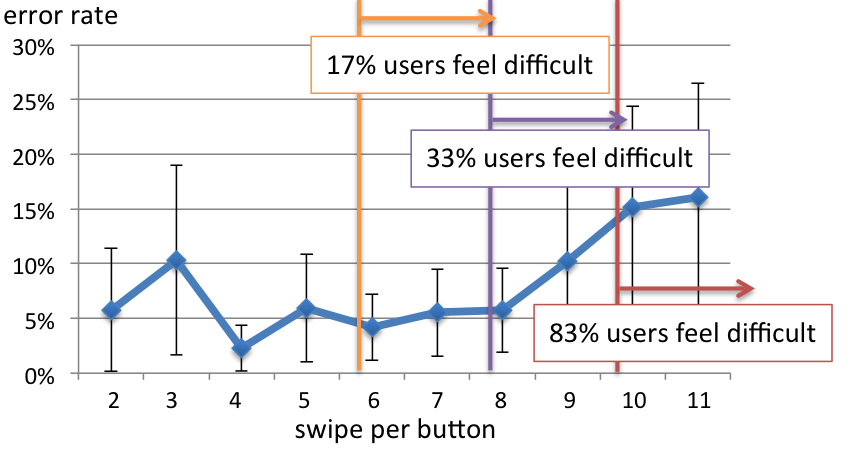
\includegraphics[width=.8\columnwidth]{figures/F6-2.png}
  \caption{}
  \label{fig:f6}
  \end{subfigure}
  \caption{Result of swipe per button test. (a) Swipe speed (b) Error rate}
\end{figure}

\subsection{Button Layout}

Based on the keyboard space and a minimum of 26 entries, we can arrange many possible layouts for each swipe number of \papertitle. Each swipe number of \papertitle\ has one layout with maximum button size. The layout choices of different swipe numbers \papertitle\ are shown in Table 1.

\begin{table}[t]
  \begin{center}
  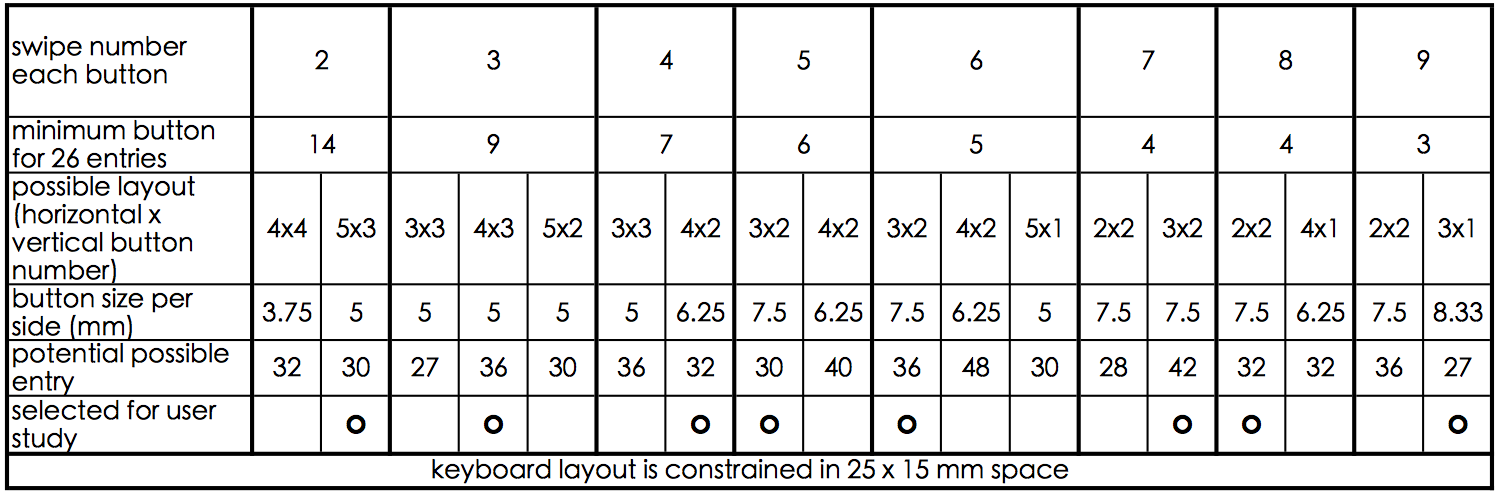
\includegraphics[width=1\columnwidth]{figures/T1.png}
  \caption[Table 1]{Layout decisions for different swipe number \papertitle. We select the layout with a largest square button size of a specific swipe number. If sizes are the same between many layouts, we then select the layout with the maximum number of potential entries.}
  \label{tab:t1}
  \end{center}
\end{table}

To investigate the influence of different swipe number layouts, we ran a user study as a continuation of our previous studies. Users were asked to swipe or tap at a random selected button and direction from 26 possible entries of 8 different types of \papertitle\ layouts. After that, users were asked to answer a questionnaire about the difficulty rating of each layout and voted for a preferred layout. Figure 6 shows the test results.

The small button size in \papertitle\ 2 and \papertitle\ 4 layouts were the worst in terms of input speed and error rate. This result is consistent with our button size user study: the error rate increases drastically if the button size is smaller than 5.7mm x 5.7mm. The large button size group also suffers a slight speed drop and error rate increase due to many possible swipe directions for each button. Although the \papertitle\ 4 and 5 layouts are the best for error rate and speed, these layouts have a nearly identical error rate and speed of \papertitle\ 6 and 7 layouts. On the other hand, user ratings paint a clearer picture. Figure 6 (c) shows that \papertitle\ 4 and 5 layouts outperform other candidates in difficulty rating and preference. Therefore, we have selected \papertitle\ 4 and 5 layouts to represent the official \papertitle\ layouts for our smartwatch text entry solution.

\subsection{Character Arrangement}
The last piece of the puzzle in designing SwipeKey is figuring out how to arrange the 26 characters in the alphabet. We considered an alphabetically ordered character layout because it is a common keyboard character layout \cite{text-entry-theory}. Secondly, there is evidence that experts typing on a keyboard with alphabetical layout perform just as well as experts typing on a QWERTY layout keyboard \cite{text-entry-theory,abc-not-matter}. Thirdly, \papertitle\ is a different type of keyboard. We did not have a proven way of transforming common keyboard layouts, such as QWERTY and Dvorak, and applying them to SwipeKey.

\begin{figure}
  \begin{subfigure}{1\columnwidth}
  \centering
  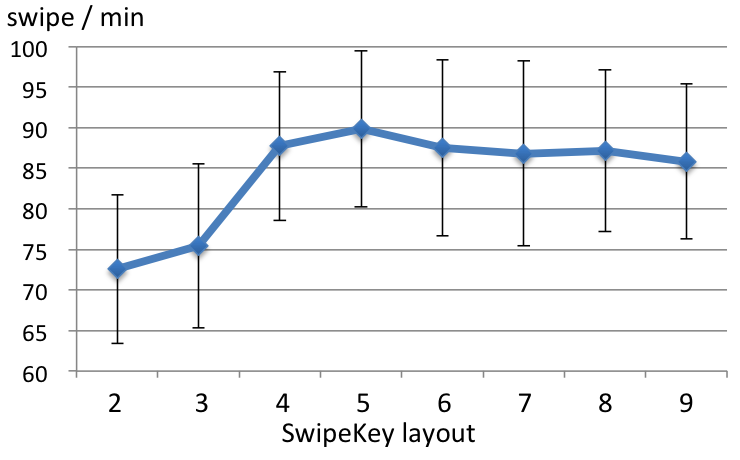
\includegraphics[width=.8\columnwidth]{figures/F7-1.png}
  \caption{}
  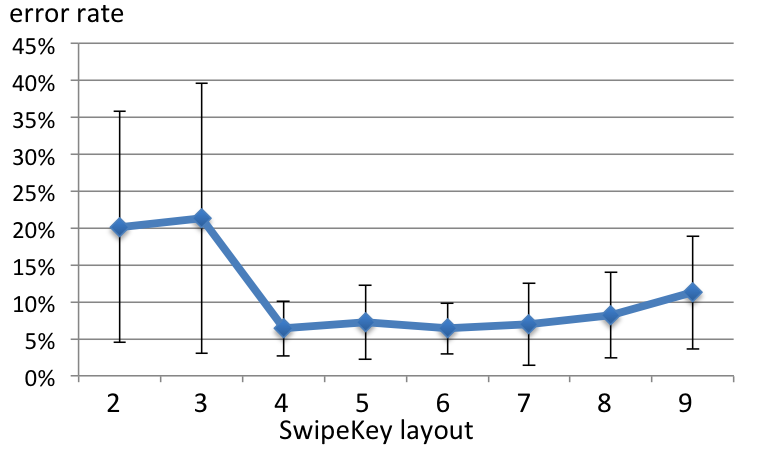
\includegraphics[width=.8\columnwidth]{figures/F7-2.png}
  \caption{}
  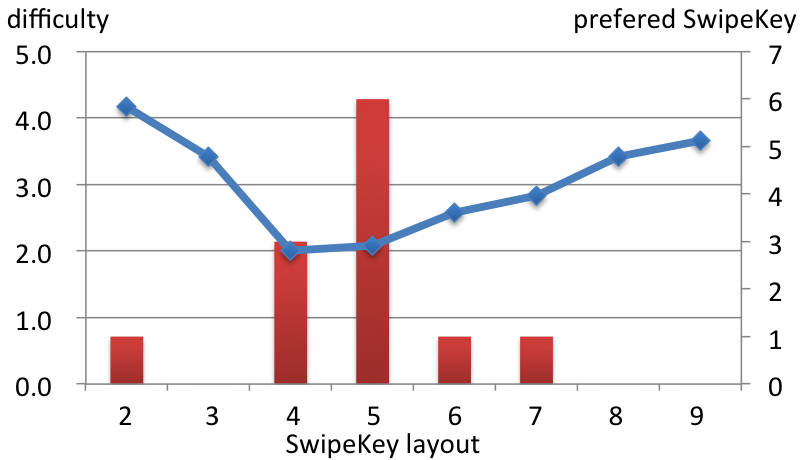
\includegraphics[width=.8\columnwidth]{figures/F7-3.png}
  \caption{}
  \label{fig:f7}
  \end{subfigure}
  \caption{Result of button layout test. (a) Test speed (b) Test error rate (c) Button layout test difficulty rating and participants preferred button layout}
\end{figure}